\section{More Complex SQL Retrieval Queries}
\subsection{Comparisons Involving NULL and Three-Valued Logic}
\textit{SQL} has some rules to manage \textbf{NULL} that can have three different interpretations:
\begin{itemize}
\item Unknown value;
\item Unavailable or withheld value;
\item Not applicable attribute.
\end{itemize}
It's often hard to detemine this interpretation. Each individual \textbf{NULL} is different. When we apply a comparison operation on a tuple which has a \textbf{NULL} value, the result is \textbf{UNKNOWN}. The figure \ref{7-1} show how logical operators are used with \textbf{UNKNOWN}:
\begin{figure}[H]
    \centering
    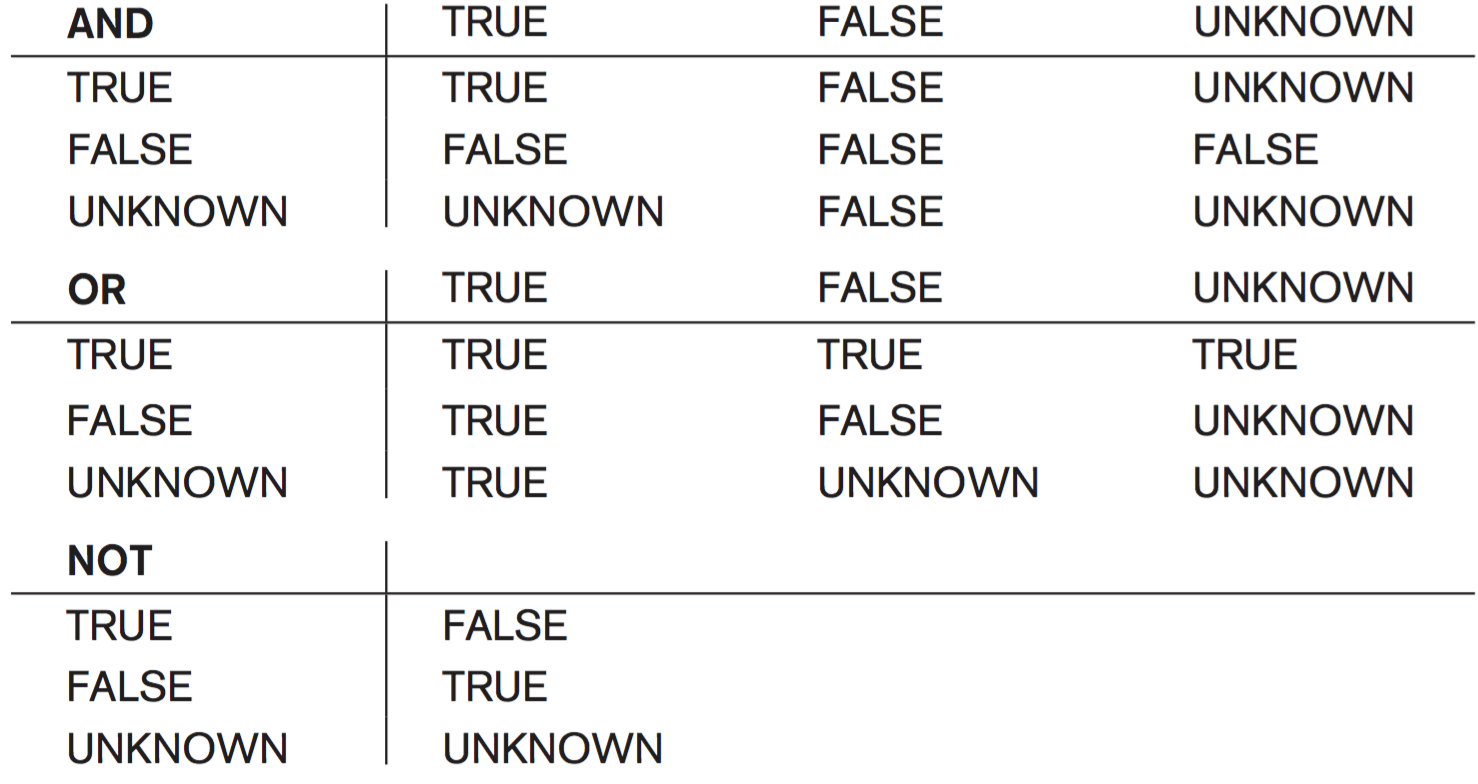
\includegraphics[scale = 0.5]{img/chap7-1}
    \caption{Logical table with \textbf{UNKNOWN}}
    \label{7-1}
\end{figure}
\textbf{UNKNOWN} is not kept in the result.
\subsection{Nested Queries, Tuples, and Set/Multiset Comparisons}
Some queries require that existing values in the database be fetched and then used in a comparison condition. To achieve it, we use Nested queries, they are complete \textit{SQL} requests within another \textit{SQL} query, called the outer query. The nested query can appear in any part of the outer query (\textbf{SELECT}, \textbf{FROM}, \textbf{WHERE}). We need to introduce the comparison operator \textbf{IN} which compare a value (or a tuple) with a set, return \textbf{TRUE} if the value is in the set.

If a nested query returns a single attribute and a single tuple, the query result will be a single value. In this case we can use "=" instead of \textbf{IN}. The = ANY (or = SOME) operator returns TRUE if the value is equal to some value in the set and is hence equivalent to \textbf{IN}. The keyword \textbf{ALL} can also be combined with each of these operators. These operators can be use with logical operators ($>,<, =, ...$)

\subsection{Correlated Nested Queries}
Whenever a condition in the \textbf{WHERE} clause of a nested query references some attribute of a relation declared in the outer query, the two queries are said to be correlated. We can understand a correlated query better by considering that the nested query is evaluated once for each tuple (or combination of tuples) in the outer query.
\subsection{The EXISTS and UNIQUE Functions in SQL}
\textbf{EXISTS} and \textbf{UNIQUE} are Boolean constraints to check if the result set of a nested query is empty or if it is unique, respectively. You can take the opposite with the keyword \textbf{NOT}

\subsection{Explicit Sets and Renaming in SQL}
You can use explicit set with \textbf{IN}. (...\textbf{WHERE} value \textbf{IN} (1,2,3 )).
You can rename what you want in \textbf{SELECT} and \textbf{FROM}. (The new name in \textbf{FROM} can be use in the corresponding \textbf{SELECT}).
\subsection{Joined Tables in SQL and Outer Joins}
You can join two tables with the instruction \textbf{JOIN ON}, that join two tables on an attribute. This instruction is done in the \textbf{FROM}. There is different type of \textbf{JOIN}:
\begin{itemize}
\item \textbf{NATURAL JOIN}: No join condition (no \textbf{ON}...), we can rename the result;
\item \textbf{INNER JOIN}: Default one, A tuple of a relation will be in the result only if it match a tuple in the other relation;
\item \textbf{OUTER JOIN}: There is a lot of different outer join: (\textbf{LEFT}(every tuple in the left table must appear in the result; if it does not have a matching tuple, it is padded with NULL values for the attributes of the right table), \textbf{RIGHT, FULL})
\item \textbf{CROSS JOIN}: Cartesian product.
\end{itemize}
\subsection{Aggregate Functions in SQL}
The aggregate functions, as \textbf{COUNT, SUM, MAX, MIN,} and \textbf{AVG} are used to summarize information and must be used in the \textbf{SELECT} statement. They return numeric values. You can refer to the row with * (\textbf{COUNT}(*) will return the number of row of the result query). Don't forget to use \textbf{DISTINCT} to discard duplicate results.
\subsection{Grouping: The GROUP BY and HAVING Clauses}
In many cases we want to apply the aggregate functions to subgroups of tuples in a relation, where the subgroups are based on some attribute values. We need to partition the relation in nonoverlaping subsets. Each subset will have the same value on the grouping attribute(s). We use \textbf{GROUP BY} to achieve it. The aggregate function will be computed for each subsets.

\textbf{HAVING} provides a condition on the summary information regarding the group of tuples associated with each value of the grouping attributes. Only the groups that satisfy the condition are retrieved in the result of the query, it must be use with \textbf{GROUP BY}.

\subsection{Other SQL Constructs: WITH and CASE}
\textbf{WITH} define a table that will only be used only in that query (quiet similar to a view). 

\textbf{CASE} can act differently due to different conditions, it can be usefull in an update operation for exemple. 
\textbf{UPDATE} table \textbf{SET} row = \textbf{CASE WHEN} condtion \textbf{THEN} ...
\subsection{Recursive Queries in SQL}
It's possible to specify recursive query in a declarative way. You may use \textbf{WITH RECURSIVE}.

\subsection{Discussion and Summary of SQL Queries}
It is possible to have six different clause in an \textit{SQL} query (\textbf{SELET, FROM, WHERE, GROUP BY, HAVING, ORDER BY}) but only \textbf{SELECT, FROM} are mandatory. 



\section{Specifying Constraints as Assertions and Actions as Triggers}
\subsection{Specifying General Constraints as Assertions in SQL}
In \textit{SQL}, we can specify general constraint (via declarative assertion) by using \textbf{CREATE ASSERTION}. Each assertion has a name and a condition (like in \textbf{WHERE}): \textbf{CREATE ASSERTION} name \textbf{CHECK} condition. The condition must be true for every database state to satisfy the assertion. The DBMS is responsible for ensur- ing that the condition is not violated.

The basic technique for writing such assertions is to specify a query that selects any tuples that violate the desired condition. By including this query inside a \textbf{NOT EXISTS} clause, the assertion will specify that the result of this query must be empty so that the condition will always be \textbf{TRUE}. Thus, the assertion is violated if the result of the query is not empty. 
\subsection{Introduction to Triggers in SQL}
Triggers are really important in \textit{SQL}, you can create them with \textbf{CREATE TRIGGER}. A trigger execute an action (a procedure or trigger other update) when a specify event appears. A trigger has three components:
\begin{itemize}
\item The event: specified by \textbf{BEFORE/AFTER INSERT/UPDATE OF };
\item The condition: determines whether the rule action should be executed (if no condition, it appears once the event appears), specified by \textbf{WHEN};
\item The action: it could be procedure, \textit{SQL} code, ...
\end{itemize}
Triggers can be used in various applications, such as maintaining database consistency, monitoring database updates, and updating derived data automatically.

\section{Views (Virtual Tables) in SQL}
\subsection{Concept of a View in SQL}
In \textit{SQL} a view is a virtual table derived from other tables taht can be real table or other views.
We can think of a view as a way of specifying a table that we need to reference frequently.

\subsection{Specification of Views in SQL}
We create a view this way: \textbf{CREATE VIEW} name[(columns names)] \textbf{AS} \textit{SQL} request. If the columns name are not specifier, they inherits the names of the attributes in the original table. A view is always up-to-date (done by DBMS). You can delete a view with \textbf{DROP VIEW} name.

\subsection{View Implementation, View Update, and Inline Views}
There is two approaches for the DBMS to implement an efficient view for querying:
\begin{itemize}
\item Query modification: modifying the view query onto queries on the base tables. Inefficient for hard requests (a lot of base table or view involved);
\item View materialization: Create physically a temporary/persistent view table, bit it needs to be up-to-date. Incremental update have been developed for this purpose, where the DBMS can determine what new tuples must be inserted, deleted, or modified in a materialized view table when a database update is applied to one of the defining base tables. There are different update: immediate, lazy (when we query on the view), periodic (may get a result that is not up-to-date).
\end{itemize}
In many case, querying \textbf{INSERT, DELETE, UPDATE} in a view isn't possible. In general, an update on a view defined on a single table without any aggregate functions can be mapped to an update on the underlying base table under certain conditions. If there is join it is often not possible for the DBMS to determine which of the updates is intended. Update a view is possible, if there is only one way to make the update in the base table.

\subsection{Views as Authorization Mechanisms}
We will use views to hide some information to unauthorized people. 

\section{Schema Change Statements in SQL}
\subsection{The DROP Command}
\textbf{DROP}can be used to drop named schema elements, tables, domains, types, or constraints. \textbf{DROP SCHEMA} drop an entire schema. There is two options parameters:
\begin{itemize}
\item \textbf{RESTRICT}: delete a schema only if it empty and a table only if there is no references in any constraints;
\item \textbf{CASCADE}: delete all the elements that have a reference to the one we want to drop.
\end{itemize}

\subsection{The ALTER Command}
For base tables, the possible alter table actions include adding or dropping a column (attribute), changing a column definition, and adding or dropping table constraints. If we add a column and no default rule is used, all the relation will have a \textbf{NULL} value.
To drop a column we must use \textbf{CASCADE} or \textbf{RESTRICT}.

\section{Summary}
In this chapter, we have described: \textbf{CREATE ASSERTION}, allows the specification of more general constraints on the database; 
\textbf{CREATE TRIGGER}, that create a trigger, piece of code launch when a specific action appears; \textbf{CREATE VIEW}, create virtual table, used for frequently used table or to give only the information allowed for users; \textbf{SQL ALTER TABLE} statement, which is used for modifying the database tables and constraints. The figure \ref{7-2} summarize all the \textit{SQL} possible type of requests.
\begin{figure}[H]
    \centering
    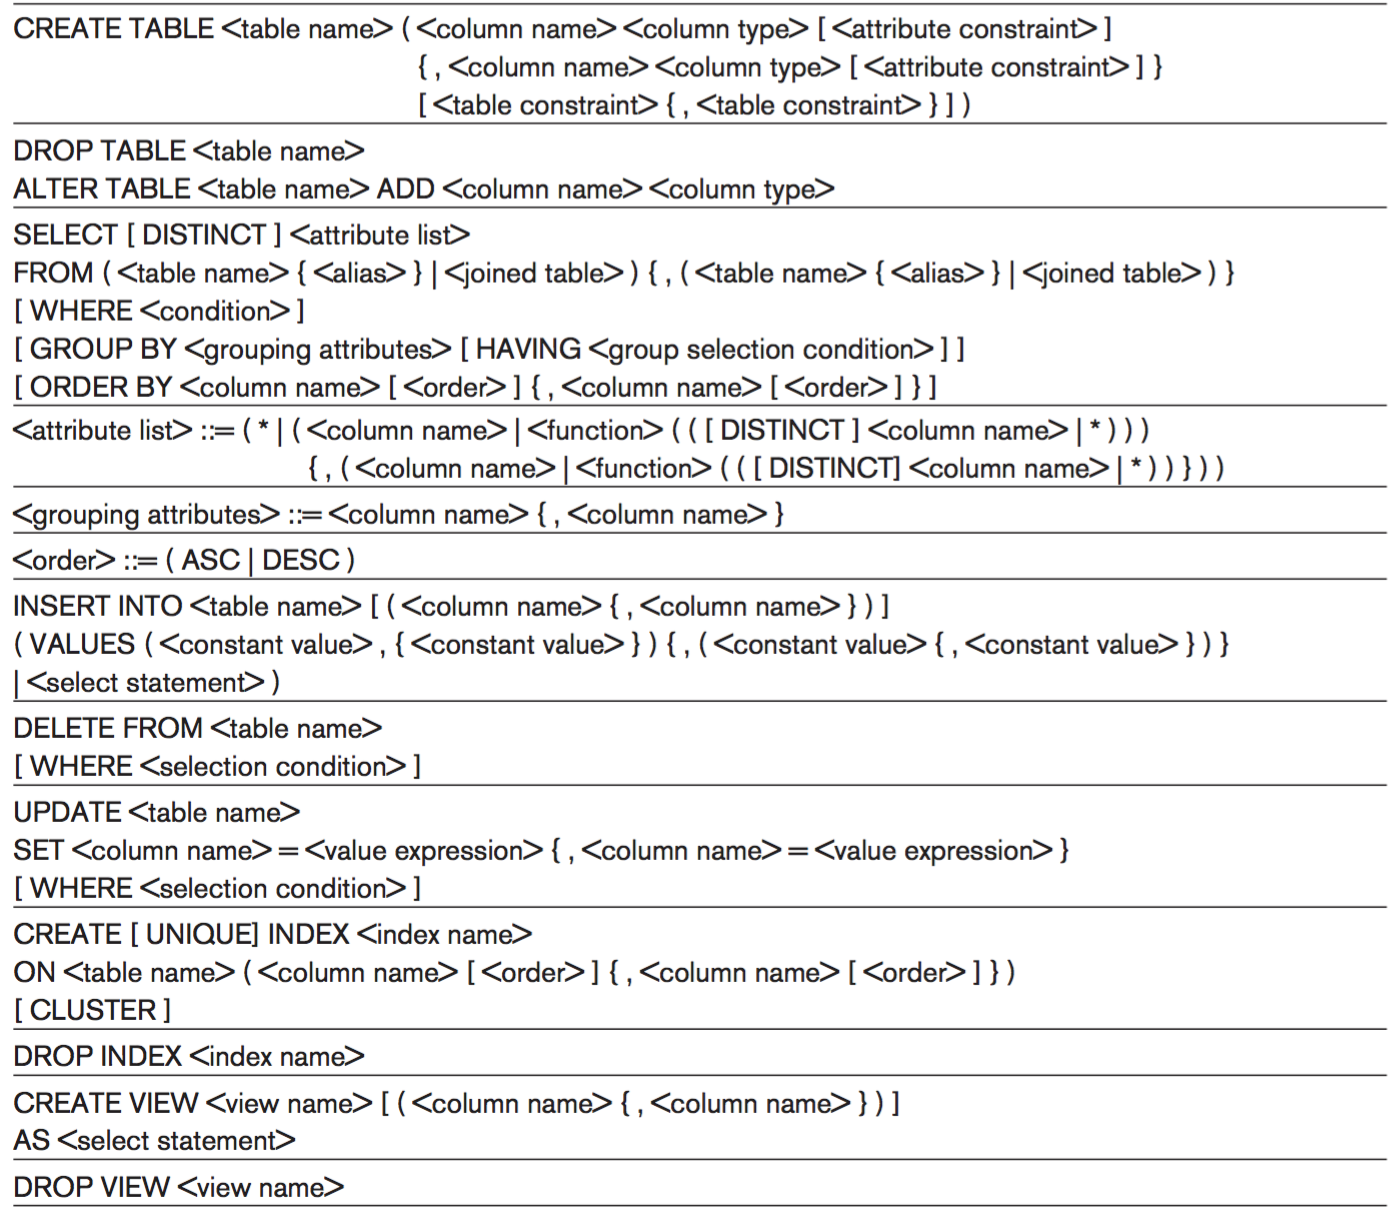
\includegraphics[scale = 0.5]{img/chap7-2}
    \caption{summary of \textit{SQL} requests.}
    \label{7-2}
\end{figure}
